\subsection{Præsentation af designet}
\begin{frame}
\frametitle{Overordnet}
\begin{center}
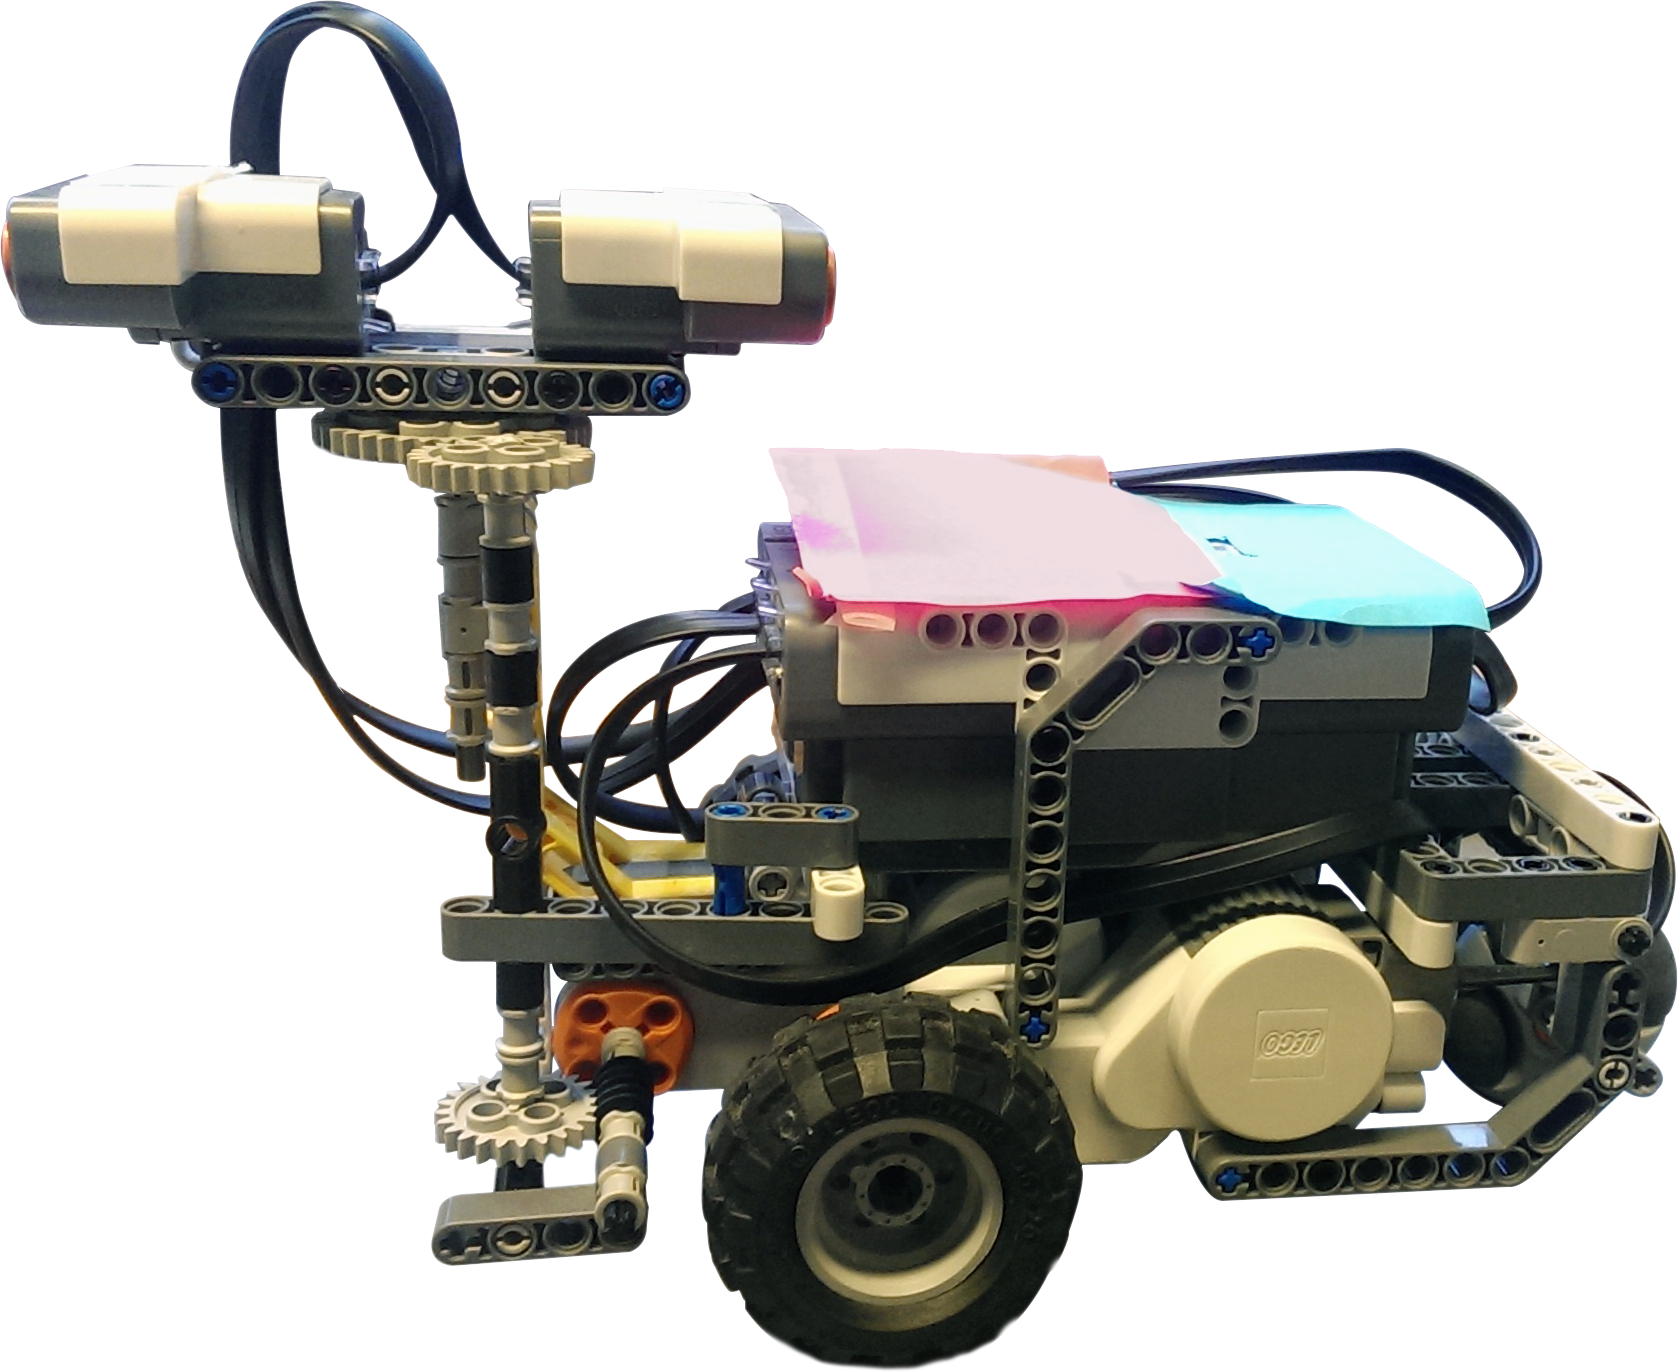
\includegraphics[scale=0.15]{whalle}
\end{center}
\end{frame}

\begin{frame}
\frametitle{Gearing}
\begin{center}
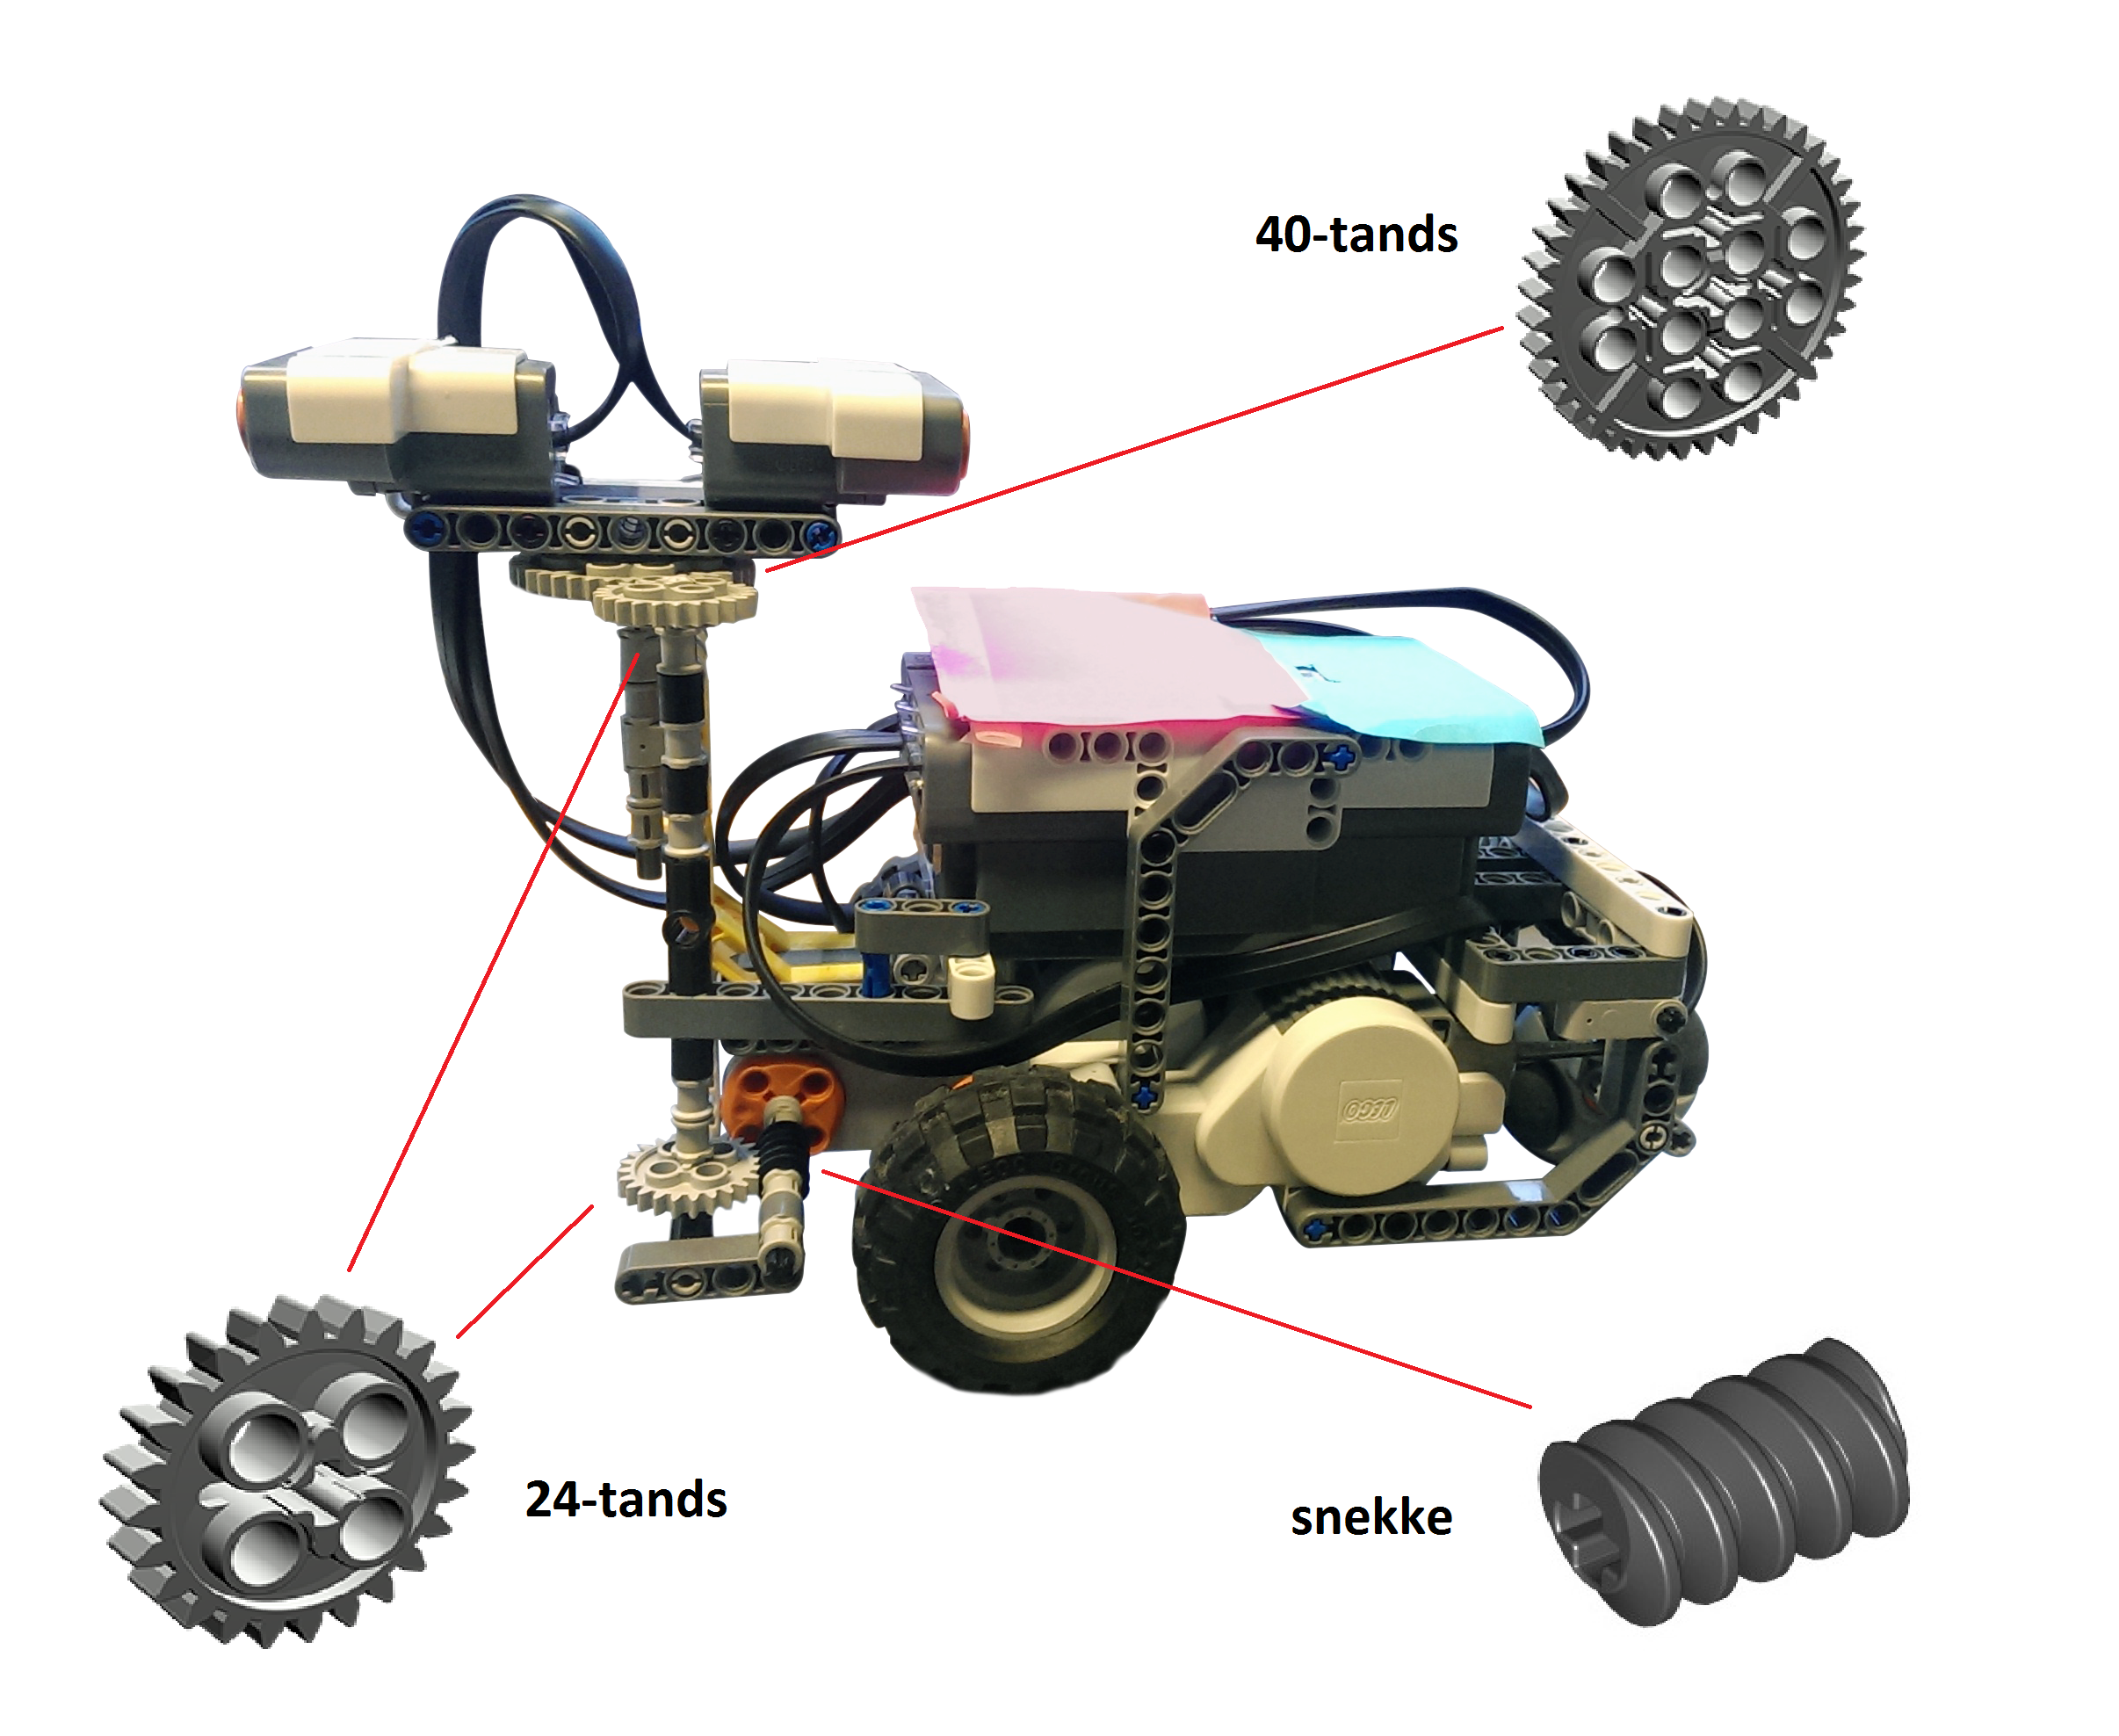
\includegraphics[scale=0.13]{whalle_with_gearing_expl}
\end{center}

\end{frame}

\subsection{Overvejelser}
\begin{frame}
\frametitle{Gearing}
\begin{itemize}
\item Gearing på hjul blev fjernet
\item Mere simpelt design
\item Unødvendigt med tårn til sensorer
\item En simplere løsning:
\begin{itemize}
\item Montere sensoren direkte på robottens krop
\item Rotere robotten når der skal måles
\end{itemize} 
\item Mindre kompleks robot design er formentlig lettere at arbejde med
\end{itemize}
\end{frame}


